\documentclass[11pt,a4paper]{report}
\usepackage[portuges]{babel}
\usepackage[utf8]{inputenc} % define o encoding usado texto fonte (input)--usual "utf8" ou "latin1
\usepackage{graphicx} %permite incluir graficos, tabelas, figuras
\usepackage{subcaption}
\usepackage[title]{appendix}
\usepackage{listings}
\usepackage{color}
\usepackage{multicol}
\usepackage{indentfirst}
\usepackage{hyperref}
\usepackage{amsmath}
\usepackage{amssymb}
\usepackage{float}
\usepackage{enumerate}
\usepackage[shortlabels]{enumitem}
\usepackage[T1]{fontenc}
\usepackage{hyperref}



\definecolor{mygreen}{rgb}{0,0.6,0}
\definecolor{mygray}{rgb}{0.5,0.5,0.5}
\definecolor{mymauve}{rgb}{0.58,0,0.82}

\hypersetup{
    colorlinks=true,
    linkcolor=blue,
    urlcolor=black,
    }
    
    
    
\usepackage{bera}% optional: just to have a nice mono-spaced font

\definecolor{eclipseStrings}{RGB}{42,0.0,255}
\definecolor{eclipseKeywords}{RGB}{127,0,85}
    

\lstset{ %
  backgroundcolor=\color{white},   % choose the background color
  basicstyle=\footnotesize,        % size of fonts used for the code
  breaklines=true,                 % automatic line breaking only at whitespace
  captionpos=b,                    % sets the caption-position to bottom
  commentstyle=\color{mygreen},    % comment style
  escapeinside={\%*}{*)},          % if you want to add LaTeX within your code
  keywordstyle=\color{blue},       % keyword style
  stringstyle=\color{mymauve},     % string literal style
}



\title{POO - Trabalho Prático\\
	\large Grupo nº5}

\author{Simão Pedro Batista Caridade Quintela \\ (A97444) 
             \and Pedro Alexandre Silva Gomes \\ (A91647)
             \and Gonçalo da Silva \\ (A95696)
       } %autores do documento
       
\date{\today} %data

\begin{document}
	\begin{minipage}{0.9\linewidth}
        \centering
		
\includegraphics[width=0.4\textwidth]{um.jpg}\par\vspace{1 cm}
		\href{https://www.uminho.pt/PT}
		{\scshape\LARGE Universidade do Minho} \par
		\vspace{0.6cm}
		\href{https://lcc.di.uminho.pt}
		{\scshape\Large Licenciatura em Ciências da Computação} \par
		\maketitle
		\begin{figure}[H]
			
\includegraphics[width=0.32\linewidth]{quintela.jpg}
			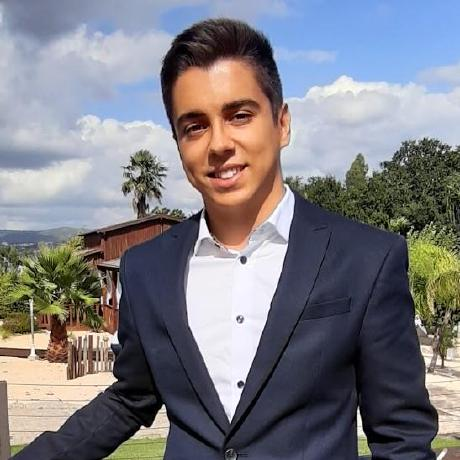
\includegraphics[width=0.32\linewidth]{pedro.jpg}
    		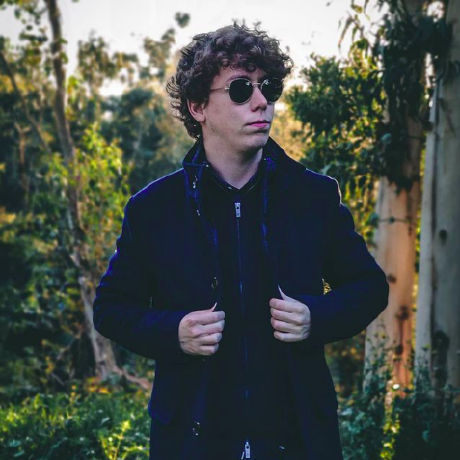
\includegraphics[width=0.32\linewidth]{goncalo.png}
		\end{figure}
	\end{minipage}
	
	\tableofcontents
	
	\pagebreak
	
	\chapter{Introdução}
%	
	Este relatório descreve o desenvolvimento do projeto prático da Unidade Currícular de Programação Orientada aos Objetos, inserida no 2ºano da Licenciatura em Ciências da Computação da Universidade do Minho.
	
	Este trabalho consistia no desenvolver de um sistema que monitorize e registe a informação sobre o consumo
energético das habitações de uma comunidade. Em cada casa existem um conjunto muito alargado de dispositivos que são todos controlados a partir deste programa, os \textit{SmartDevice}. Para que a realização do referido fosse possível, utilizamos os conhecimentos da linguagem \textit{Java}, adquiridos ao longo do semestre.  
	
	\pagebreak
	\chapter{Classes}
	
	Estas são as classes que constituem o nosso programa:
	
    \section{App}
    \begin{lstlisting}[language=java,firstnumber=1]
    static Scanner scan = new Scanner(System.in);
    static Comunidade comunidade = new Comunidade("Jackson");
    static Controller controller = new Controller(comunidade);
    \end{lstlisting}
    
	\section{CasaInteligente}
	\subsection{CasaInteligente}
	\begin{lstlisting}[language=java,firstnumber=1]
    private String proprietario;
    //private int numeroDePorta;
    private int NIF;
    //private String morada;
    private String fornecedor;
    private Map<String, SmartDevice> devices; // identificador -> SmartDevice
    private Map<String, List<String>> locations; // Espaço -> Lista codigo dos devices
    private List<Fatura> faturas; // lista de faturas que foram geradas e associadas à casa
    \end{lstlisting}
    
	\subsection{CasaInteligenteTest}
	\subsection{SmartDevices}
        \begin{itemize}
        \item SmartDevice
        \begin{lstlisting}[language=java,firstnumber=1]
    private String id;
    private boolean on;
    private LocalDate time;
    private float consumption;
    private float consumptionPerDay;
    private int custoInstalacao;
    \end{lstlisting}
    
        \item SmartDeviceTest
        \item SmartBulb
        \begin{lstlisting}[language=java,firstnumber=1]
    private static final int WARM = 80;
    private static final int NEUTRAL = 60;
    private static final int COLD = 40;
    private int tone;
    private int dimensions;
    \end{lstlisting}
    
        \item SmartBulbTest
        \item SmartSpeaker
        \begin{lstlisting}[language=java,firstnumber=1]
    private static final int MAX = 100; //volume maximo
    private int volume;
    private String channel;
    private String brand;
    \end{lstlisting}
    
        \item SmartCamera
        \begin{lstlisting}[language=java,firstnumber=1]
    private int xRes;
    private int yRes;
    private int fileSize;
    private float custoInstalacao;
    \end{lstlisting}
    
        \end{itemize}
        
	\section{ComercializadoresEnergia}
	
	\subsection{Comercializador}
	\begin{lstlisting}[language=java,firstnumber=1]
    private String nomeEmpresa;
    private int numeroDispositivos;
    private int valorBase;
    private int imposto;
    private Map<String, List<Fatura>> faturas;  // Proprietário -> Lista de Faturas
    //private double precoDiaPorDispositivo = numeroDispositivos > 10?(valorBase * consumoDispositivo * (1 + imposto)) * 0.9 : (valorBase * consumoDispositivo * (1 + imposto)) * 0.75;
    \end{lstlisting}
	
	\subsection{Fatura}
	\begin{lstlisting}[language=java,firstnumber=1]
    private int codigo;
    private int nif;
    LocalDate dataEmissao;
    private Map<String, Float> consumoDevice; //id -> consumo
    private String empresa;
    private String cliente;
    \end{lstlisting}
	
	\section{Comunidade}
	\begin{lstlisting}[language=java,firstnumber=1]
    private String nomeDaComunidade;
    private Map<String, CasaInteligente> casas;
    private Map<String, Comercializador> mercado;
    \end{lstlisting}
	
	\section{Controller}
	\begin{lstlisting}[language=java,firstnumber=1]
    private Comunidade comunidade;
    private int idFatura;
    private LocalDate timeNow;
    \end{lstlisting}
	
    \section{Parser}
    
    \section{SaveProgramText}
    
    \section{SimulParser}
    
    \section{View}
    \begin{lstlisting}[language=java,firstnumber=1]
    private Controller controller;
    private Scanner scan;
    \end{lstlisting}
    
	\pagebreak
	
	\section{Diagrama de classes do \textit{blueJ}}
	
	\begin{figure}[H]
			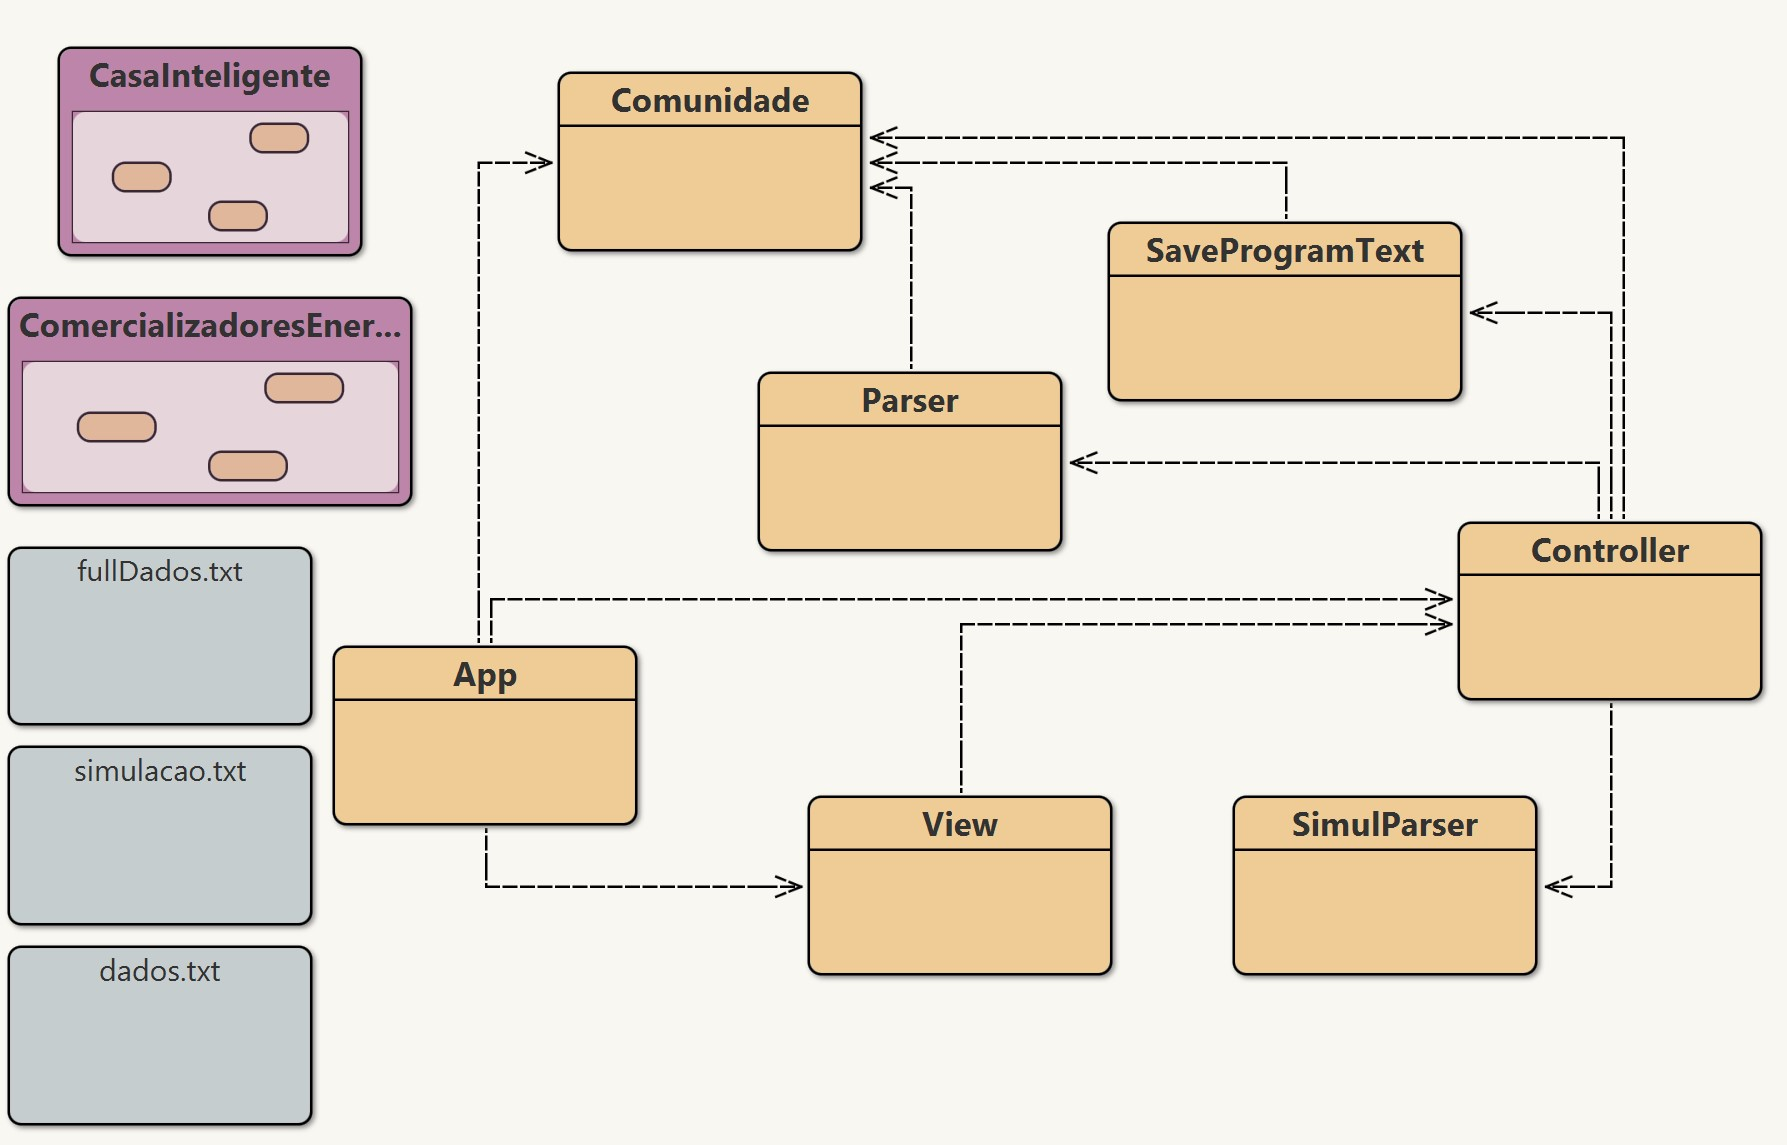
\includegraphics[scale=0.8]{diagrama1.jpg}
	\end{figure}
	
\begin{enumerate}
    \item Diagrama principal com as super classes, interfaces de simulação e ficheiros .txt
    \vspace{13mm} %5mm vertical space

	\begin{figure}[H]
			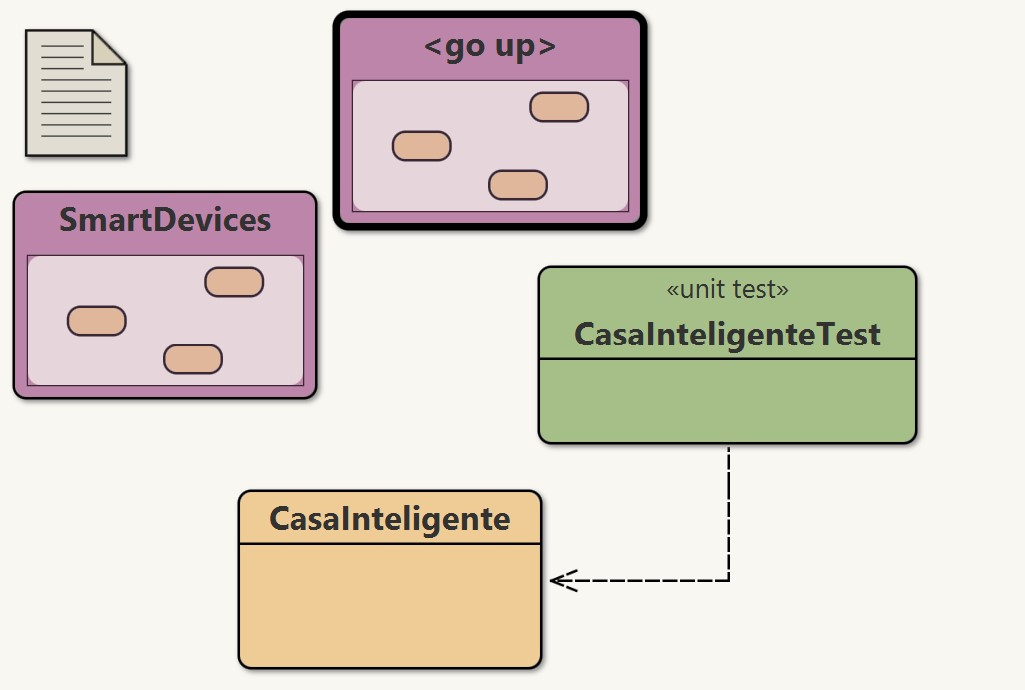
\includegraphics[scale=0.8]{diagrama2.jpg}
	\end{figure}
	
\item Diagrama da classe CasaInteligente
\vspace{15mm} %5mm vertical space

	\begin{figure}[H]
    		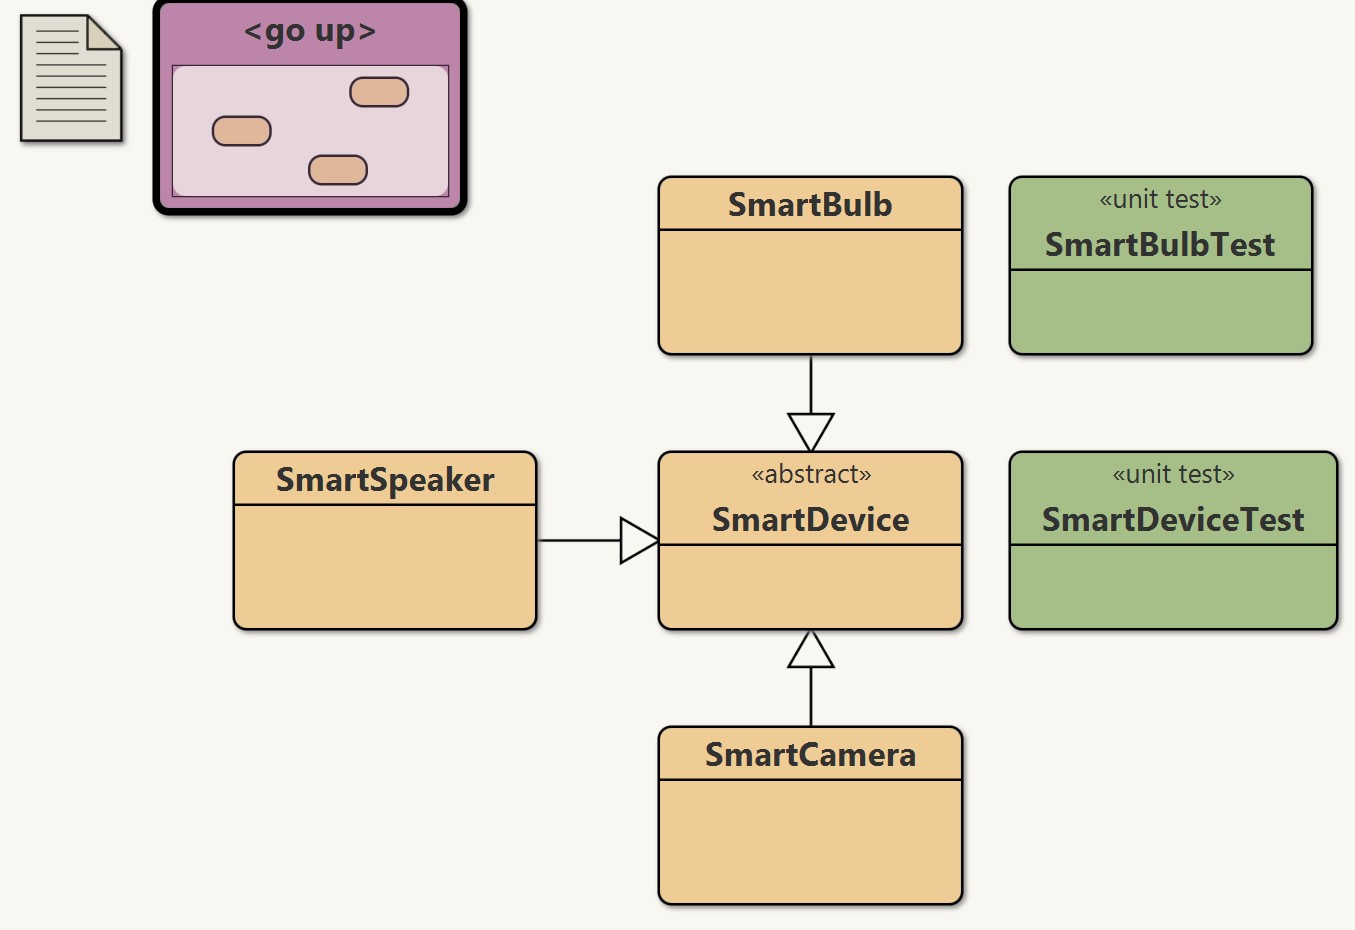
\includegraphics[scale=0.8]{diagrama3.jpg}
    \end{figure}
    
\item Diagrama da classe SmartDevices 
\vspace{15mm} %5mm vertical space

    \begin{figure}[H]
    		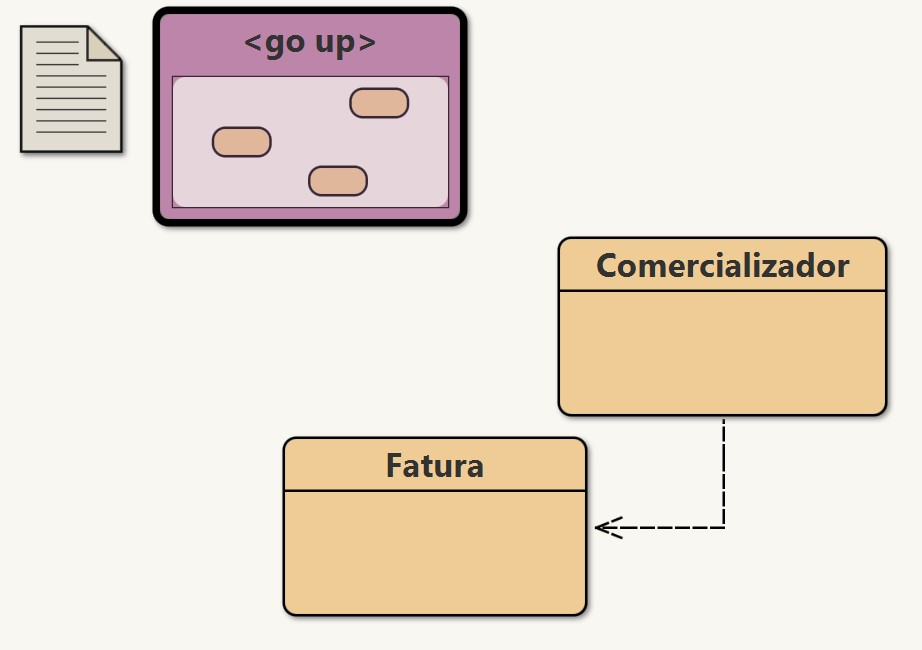
\includegraphics[scale=0.8]{diagrama4.jpg}
	\end{figure}
	
\item Diagrama da classe ComercializadoresEnergia

\end{enumerate}
    \pagebreak

\chapter{Estrututa do projeto}

O nosso projeto segue o modelo de estrutura \textbf{\textit{Model View Controller} (MVC)}, que consite na organização deste em três camadas:
	\begin{itemize}
		\item A camada de dados \textbf{(o modelo)} é composta pelas classes CasaInteligente, SmartDevice, SmartBulb, SmartSpeaker, SmartCamera, Comercializador, Fatura, Comunidade e a pelas interfaces de Simulação.
		\item A camada de interação com o utilizador \textbf{(a vista, ou apresentação)} é composta unicamente pela classe View.
		\item A camada de controlo do fluxo do programa\textbf{ (o controlador)} é composta pela classe Controller.
	\end{itemize}
        Em todo o projeto respeitamos a ideia de encapsulamento, como pedido.


\pagebreak

\chapter{Diagrama do \textit{Intellij}}
\begin{figure}[H]
			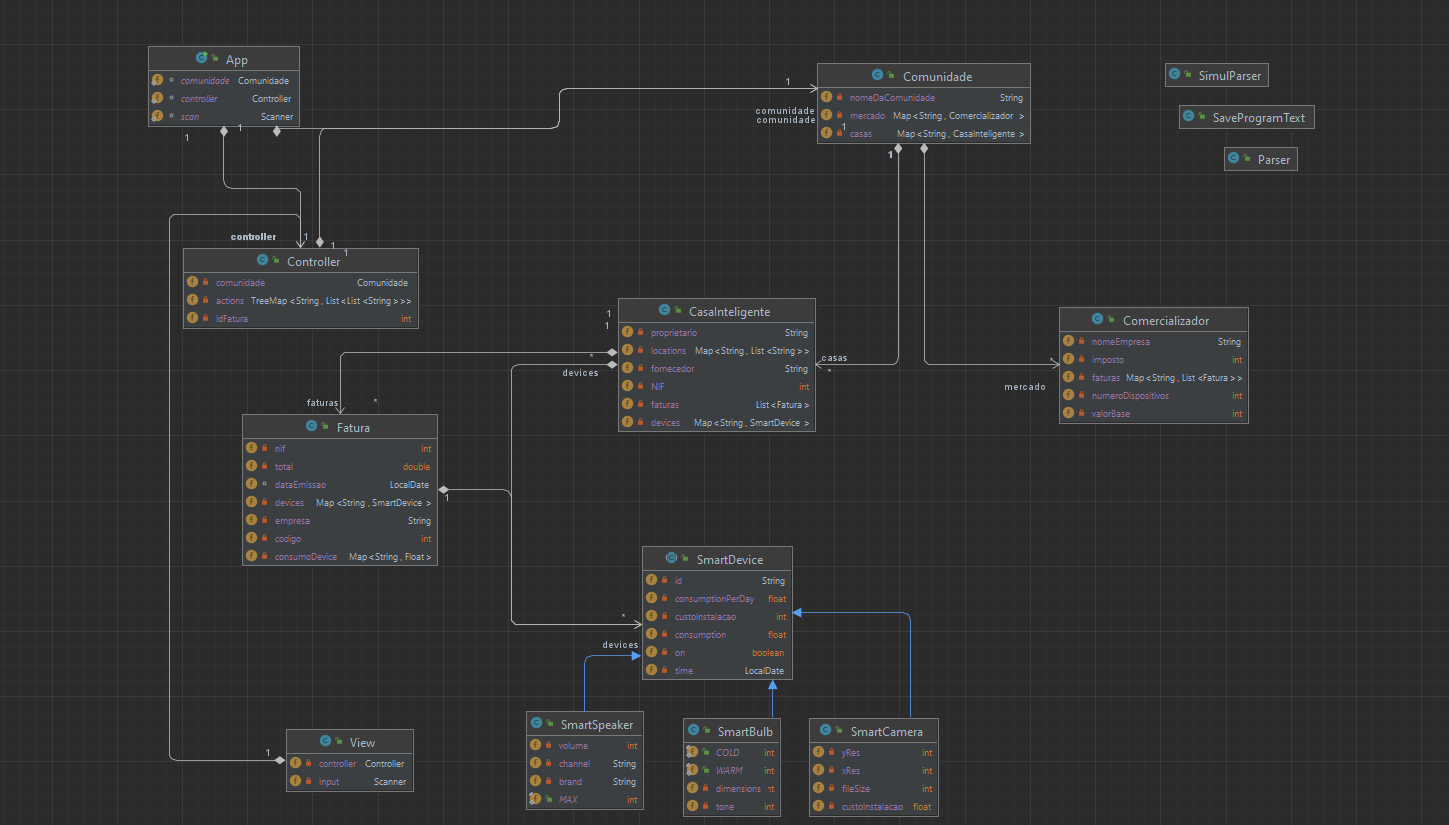
\includegraphics[scale=0.30]{diagramaIntellij.jpg}
	\end{figure}
    
    
\pagebreak	
	\chapter{Conclusão}
    
    Em conclusão, a nível geral, e tendo em conta o panorama apresentado nos capítulos anteriores e os objetivos pedidos para esta realização, como grupo, achamos que todos os objetivos foram cumpridos, conseguindo superar com sucesso, todas as dificuldades que fomos encontrando,  sempre com um olhar crítico e empenhados. Acreditamos que aprendemos os conteúdos e objetivos desta Unidade Curricular e em particular deste projeto.
	

\end{document}

